\documentclass[a4paper]{article}
\usepackage[utf8x]{inputenc}
\usepackage[lastexercise]{exercise}
\usepackage{color}
\usepackage[absolute]{textpos} 
\usepackage{verbatim}
\usepackage{tikz}
\usetikzlibrary{calc}
\usetikzlibrary{positioning}

\renewcommand\ExerciseName{Exercice}
\renewcommand{\AnswerHeader}{\medskip\centerline{\textbf{Solution de
                        l'\ExerciseName  \ExerciseHeaderNB}\smallskip}}
\newenvironment{CAnswer}{\color{red}\begin{Answer}}
                        {\end{Answer}}



\title{Prolog - TP1\\Représentation de problèmes, Unification}
\date{}

\begin{document}
\maketitle
\begin{textblock*}{4cm}(10mm,10mm)
\begin{Large}ESIAL 3A IL LE\end{Large}
\end{textblock*}
\begin{textblock*}{3cm}(160mm,10mm)

\includegraphics[width=\textwidth]{../../ESIAL.pdf}
\end{textblock*}

\section*{Mise en route:}
\begin{itemize}
 \item lancez GNU Prolog à l'aide de la commande gprolog
 \item pour charger un fichier, utilisez \verb#consult/1.# Par ex 
       \verb#?­ consult('fichier.pro').# où fichier.pro doit se 
       trouver dans le répertoire de lancement. Alternativement utilisez
       \verb#?­ [fichier].# (sans l'extension).
 \item pour lister la base de connaissances, utilisez \verb#listing/0#.
 \item pour utiliser le debug, utilisez \verb#trace/0# et \verb#notrace/0#.
 \item pour arrêter, utilisez le prédicat \verb#halt/0#.
\end{itemize}

\begin{Exercise}[title={Premiers pas}]
\Question Représentez les assertions suivantes en prolog :
\subQuestion Harry est un magicien
\subQuestion Hagrid fait peur à Dudley
\subQuestion Tous les magiciens sont magiques
\subQuestion L'oncle Vernon déteste tout ce qui est magique
\subQuestion La tante Pétunia déteste tout ce qui est magique ou
             fait peur à Dudley

\Question Vérifiez votre programme en testant les requêtes :
\subQuestion Est­ce que Pétunia déteste Hagrid ? (oui)
\subQuestion Qui l'oncle Vernon déteste­t'il ? (Harry)
\subQuestion Qui la tante Pétunia déteste­t'elle ? (Harry et Hagrid,
             utilisez le point virgule pour avoir la seconde solution).
\end{Exercise}
\begin{CAnswer}
\verbatiminput{premiers_pas.pro}
\end{CAnswer}

\begin{Exercise}[title={Puzzle}]
On cherche toutes les façons de placer dans une grille de mots croisés les
mots : \emph{abalone}, \emph{abandon}, \emph{anagram}, \emph{connect},
\emph{elegant}, \emph{enhance}. Vous devez définir une règle de prédicat 
\verb#puzzle/6# dont les trois premiers arguments sont les mots dans les
colonnes V1,V2,V3, et les trois suivants sont les mots dans les lignes 
H1,H2,H3. Vous vous appuierez sur la base de connaissances ci-­dessous. Vous 
pourrez éventuellement utiliser la variable anonyme (\verb#_#) pour simplifier
l'écriture de la règle\footnote{la variable anonyme est une variable muette
qui n'est pas retournée et qu'on peut utiliser plusieurs fois dans une règle 
sans coréférence (plusieurs variables anonymes peuvent coexister dans une 
règle sans imposer la même valeur).}.

\begin{minipage}{.5\textwidth}
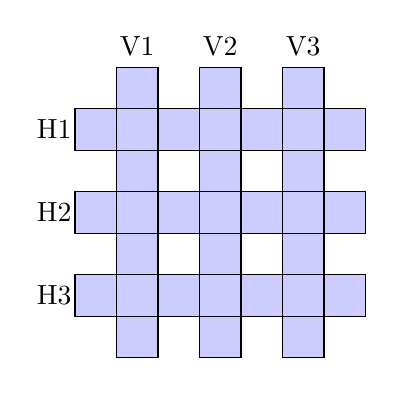
\begin{tikzpicture}[node distance=1.5em]
 \matrix[nodes={draw, fill=blue!20, minimum size=1.5em},
        row sep=-0.4pt,column sep=-0.4pt]{
             & \node(v1){}; &          & \node(v2){}; &
                                       & \node(v3){}; &           \\
\node(h1){}; & \node    {}; & \node{}; & \node    {}; &
                              \node{}; & \node    {}; & \node{};\\
             & \node    {}; &          & \node    {}; &
                                       & \node    {}; &           \\
\node(h2){}; & \node    {}; & \node{}; & \node    {}; &
                              \node{}; & \node    {}; & \node{};\\
             & \node    {}; &          & \node    {}; &
                                       & \node    {}; &           \\
\node(h3){}; & \node    {}; & \node{}; & \node    {}; &
                              \node{}; & \node    {}; & \node{};\\
             & \node    {}; &          & \node    {}; &
                                       & \node    {}; &           \\
 };
\node [left of=h1] {H1};
\node [left of=h2] {H2};
\node [left of=h3] {H3};
\node [above of=v1] {V1};
\node [above of=v2] {V2};
\node [above of=v3] {V3};
\end{tikzpicture}
\end{minipage}
\begin{minipage}{.5\textwidth}
\begin{verbatim}
mot(abalone,a,b,a,l,o,n,e).
mot(abandon,a,b,a,n,d,o,n).
mot(enhance,e,n,h,a,n,c,e).
mot(anagram,a,n,a,g,r,a,m).
mot(connect,c,o,n,n,e,c,t).
mot(elegant,e,l,e,g,a,n,t).
\end{verbatim}
\end{minipage}
\end{Exercise}
\begin{CAnswer}
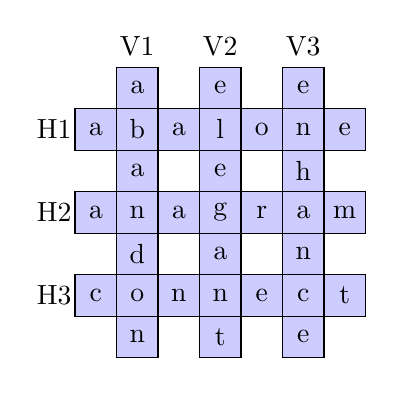
\begin{tikzpicture}[node distance=1.5em]
 \matrix[nodes={draw, fill=blue!20, minimum size=1.5em},
        row sep=-0.4pt,column sep=-0.4pt]{
              & \node(v1){a}; &           & \node(v2){e}; &
                                          & \node(v3){e}; &          \\
\node(h1){a}; & \node    {b}; & \node{a}; & \node    {l}; &
                                \node{o}; & \node    {n}; & \node{e};\\
              & \node    {a}; &           & \node    {e}; &
                                          & \node    {h}; &          \\
\node(h2){a}; & \node    {n}; & \node{a}; & \node    {g}; &
                                \node{r}; & \node    {a}; & \node{m};\\
              & \node    {d}; &           & \node    {a}; &
                                          & \node    {n}; &          \\
\node(h3){c}; & \node    {o}; & \node{n}; & \node    {n}; &
                                \node{e}; & \node    {c}; & \node{t};\\
              & \node    {n}; &           & \node    {t}; &
                                          & \node    {e}; &          \\
 };
\node [left of=h1] {H1};
\node [left of=h2] {H2};
\node [left of=h3] {H3};
\node [above of=v1] {V1};
\node [above of=v2] {V2};
\node [above of=v3] {V3};
\end{tikzpicture}
\verbatiminput{puzzle.pro}
\end{CAnswer}

\begin{Exercise}[title={Négation de l'unification}]
On a vu en cours l'unification et le prédicat \verb$=/2$ permettant de la
tester. Il peut être utile de préciser dans les règles que l'unification ne doit
pas réussir, et on peut utiliser le prédicat \verb$\=/2$ vrai lorsque \verb$=/2$
est faux. C'est­à­dire par exemple \verb$X \= Y$ est vrai lorsque \verb$X$ ne
s'unifie pas à \verb$Y$. A l'aide de ce prédicat, écrivez les règles pour
définir correctement une ligne verticale et une ligne horizontale au moyen des
prédicats \verb$verticale/1$, \verb$horizontale/1$, \verb$ligne/2$, et
\verb$point/2$. Par exemple \verb$verticale(ligne(point(1,2), point(1,3)))$.
Testez enfin : \verb$verticale(ligne(point(1,2), point(1,X)))$. Qu'observez­vous
? Etudiez le mode trace (\verb$trace/0$) de cette requête et déterminez la
raison du comportement observé.
\end{Exercise}
\begin{CAnswer}
\verbatiminput{negation.pro}
\end{CAnswer}

\begin{Exercise}[title={Généalogie}]
Modélisez la famille suivante :
\begin{center}
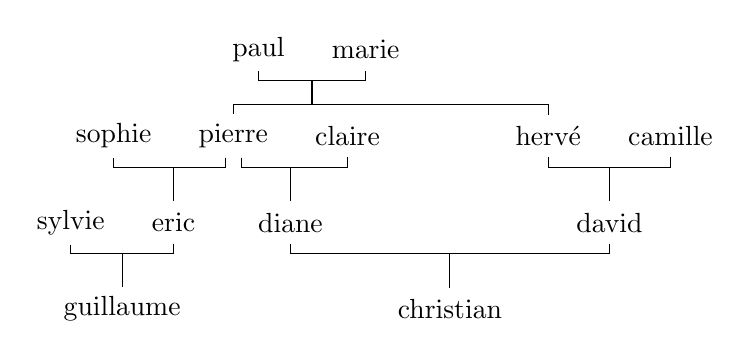
\begin{tikzpicture}[node distance=1em, nodes={minimum size=1.5em},
	      link/.style={to path={-- ++(0,#1) -| (\tikztotarget)}}]
\node (paul) {paul};
\node [right=of paul] (marie) {marie};
\coordinate (mid paul marie) at ($(paul)!.5!(marie)!.6cm!90:(paul)$);

\node (pierre) at ($(mid paul marie) + (-1cm,-.5cm)$) {pierre};
\node [right=of pierre] (claire) {claire};
\coordinate (mid pierre claire) at ($(pierre)!.5!(claire)!.6cm!90:(pierre)$);

\node [left=of pierre] (sophie) {sophie};
\coordinate (mid pierre sophie) at ($(pierre)!.5!(sophie)!.6cm!-90:(pierre)$);

\node (herve)  at ($(mid paul marie) + (3cm,-.5cm)$) {herv\'e};
\node [right=of herve] (camille) {camille};
\coordinate (mid herve camille) at ($(herve)!.5!(camille)!.6cm!90:(herve)$);

\node (eric) at ($(mid pierre sophie) + (0cm,-.5cm)$) {eric};
\node [left=of eric] (sylvie) {sylvie};
\coordinate (mid eric sylvie) at ($(eric)!.5!(sylvie)!.6cm!-90:(eric)$);

\node (diane) at ($(mid pierre claire) + (0cm,-.5cm)$) {diane};
\node (david) at ($(mid herve camille) + (0cm,-.5cm)$) {david};
\coordinate (mid david diane) at ($(david)!.5!(diane)!.6cm!-90:(david)$);

\node (guillaume) at ($(mid eric sylvie) + (0cm,-.5cm)$) {guillaume};
\node (christian) at ($(mid david diane) + (0cm,-.5cm)$) {christian};


\draw (paul) edge[link=-.4cm] (mid paul marie) edge[link=-.4cm] (marie);
\draw (pierre) edge[link=.4cm] (mid paul marie);
\draw (herve) edge[link=.4cm] (mid paul marie);
\draw ($(pierre.south) + (.1cm,0)$) edge[link=-.13cm] (mid pierre claire)
                                    edge[link=-.13cm] (claire);
\draw ($(pierre.south) + (-.1cm,0)$) edge[link=-.13cm] (mid pierre sophie)
                                     edge[link=-.13cm] (sophie);
\draw (herve) edge[link=-.4cm] (mid herve camille) edge[link=-.4cm] (camille);
\draw (eric) edge[link=.4cm] (mid pierre sophie);
\draw (diane) edge[link=.4cm] (mid pierre claire);
\draw (david) edge[link=.4cm] (mid herve camille);
\draw (eric) edge[link=-.4cm] (mid eric sylvie) edge[link=-.4cm] (sylvie);
\draw (david) edge[link=-.4cm] (mid david diane) edge[link=-.4cm] (diane);
\draw (guillaume) edge[link=.4cm] (mid eric sylvie);
\draw (christian) edge[link=.4cm] (mid david diane);
\end{tikzpicture}
\end{center}
Ecrivez ensuite les prédicats et les règles correspondant à : \verb$homme/1$,
\verb$femme/1$, \verb$pere/2$, \verb$mere/2$, \verb$parent/2$, \verb$frere/2$,
\verb$soeur/2$, \verb$oncle/2$, \verb$tante/2$, \verb$cousin/2$.

Cherchez comment il serait possible d'écrire un prédicat \verb$ancetre/2$, vrai
si le premier individu est un ancêtre du second. Ecrivez le prédicat
\verb$famille/2$, vrai si deux individus partagent un ancêtre commun. Enfin,
écrivez le prédicat \verb$consanguin/3$, vrai lorsqu'un enfant a deux parents de
la même famille.
\end{Exercise}
\begin{CAnswer}
\verbatiminput{genealogie.pro}
\end{CAnswer}

\begin{Exercise}[title={Voisinage}]
On suppose que vous êtes un peintre en bâtiment et deviez peindre trois maisons
d'une rue en sachant que la maison bleue doit être située à côté de la maison
rouge, et que la maison verte doit être située à côté de la maison bleue. 
\begin{center}
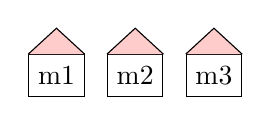
\begin{tikzpicture}[nodes={draw, minimum size=1.5em}]
 \foreach \x in {1,2,3} {
   \node (m\x) at (\x cm, 0) {m\x};
   \draw[fill=red!20] (m\x.north east) -- ($(m\x) + (0,.6cm)$) -- (m\x.north west);
 }
\end{tikzpicture}
\end{center}
Modélisez ce problème en Prolog afin de déterminer quelle maison doit être
peinte de quelle couleur. Vous définirez un prédicat \verb$couleur/3$, tel qu'il
associe à chaque argument un terme dénotant la couleur. Par exemple \verb$?­couleur(X,Y,Z).$
retournera \verb$X = rouge(m1) Y = bleu(m2) Z = vert(m3)$.
\end{Exercise}
\begin{CAnswer}
\verbatiminput{voisinage.pro}
\end{CAnswer}
\end{document}
